%%%%%%%%%%%%%%%%%%%%%%%%%%%%%%%%%%%%%%%%%%%%%%%%%%%%%%%%%%%%%%%%%%%%%%%%%%%%%%%%
%2345678901234567890123456789012345678901234567890123456789012345678901234567890
%        1         2         3         4         5         6         7         8

\documentclass[letterpaper, 10 pt, conference]{ieeeconf}  % Comment this line out if you need a4paper

%\documentclass[a4paper, 10pt, conference]{ieeeconf}      % Use this line for a4 paper

\IEEEoverridecommandlockouts                              % This command is only needed if 
                                                          % you want to use the \thanks command

\overrideIEEEmargins                                      % Needed to meet printer requirements.

% See the \addtolength command later in the file to balance the column lengths
% on the last page of the document

% The following packages can be found on http:\\www.ctan.org
%\usepackage{graphics} % for pdf, bitmapped graphics files
%\usepackage{epsfig} % for postscript graphics files
%\usepackage{mathptmx} % assumes new font selection scheme installed
%\usepackage{times} % assumes new font selection scheme installed
%\usepackage{amsmath} % assumes amsmath package installed
%\usepackage{amssymb}  % assumes amsmath package installed
\usepackage{graphicx}

%\title{\LARGE \bf Elbow Joint Angle Estimation Through The Measurement of Surface Electromyography
%}
% * <aforner@usp.br> 2018-01-28T08:34:32.702Z:
%
% ^.
\title{\LARGE \bf Elbow Joint Angle Estimation with Surface Electromyography Using Autoregressive Models
}

\author{L. F. Sommer, C. Barreira, C. Noriega, F. Camargo-Junior, R.T. Moura and A. Forner-Cordero% <-this % stops a space
\thanks{Leonardo Fischi Sommer, Caue Barreira, Carlos Noriega, Franklin Camargo-Junior, Rafael Moura and Arturo Forner-Cordero are with the Biomechatronics Laboratory, Escola Politecnica of the University of Sao Paulo, Avda Prof Mello Moraes, 2231, Sao Paulo, Brazil {\tt\small leonardo.sommer@usp.br, aforner@usp.br}}
}
\begin{document}


\maketitle
\thispagestyle{empty}
\pagestyle{empty}


%%%%%%%%%%%%%%%%%%%%%%%%%%%%%%%%%%%%%%%%%%%%%%%%%%%%%%%%%%%%%%%%%%%%%%%%%%%%%%%%
\begin{abstract}

%This paper presents a method for elbow joint angle estimation through the measurement of surface electromyography from the biceps, triceps and brachioradialis. This estimation has great importance for either mechanical modeling of biologic systems and bio-inspired mechanisms. However interpreting and processing electromyography signals is challenging due to nonlinearities, unmodeled muscle dynamics and interference signals. Here a model is proposed based on experimental data of the elbow movement and the EMG recordings of the biceps brachii, triceps brachii and brachioradialis. A system identification method is applied to estimate an Auto-Regressive Moving Average with Exogenous Input (ARMAX) model to calculate the elbow joint angle using the acquired EMG data as input to the system. The results show that the proposed model achieves great values for both correlation and mean-square-root error when compared to the measured angle data, proving to be an effective model for the EMG-to-angle relation.

This paper presents a method to estimate the elbow joint angle from surface electromyography (sEMG) measurements of biceps, triceps and brachioradialis. This estimation is of major importance for the design of human robot interfaces based on sEMG. It is also relevant to model the muscular system and to design biomimetic mechanisms. However, the processing and interpretation of electromyographic signals is challenging due to nonlinearities, unmodeled muscle dynamics, noise and interferences. In order to determine an estimation model and a calibration procedure for the model parameters, a set of experiments were carried out with six subjects. The experiments consisted of series of continuous (cyclical) and discrete elbow flexo-extensions with three different loads (i.e. 0 kg, 1.5kg and 3 kg). The sEMG data from the biceps brachii, triceps brachii and brachioradialis and the joint angle were recorded. Four different modeling techniques were evaluated: State Space (SS), Autoregressive with Exogenous Input (ARX), Autoregressive Moving-Average with Exogenous Input (ARMAX), Autoregressive Integrated Moving-Average with Exogenous Input (ARIMAX). After the model was selected, a second experiment was performed in order to validate the estimation procedure. The results show a procedure to estimate the EMG-to-angle relation with high correlation and low mean-square-root errors with respect to the measured angle data.

\end{abstract}


%%%%%%%%%%%%%%%%%%%%%%%%%%%%%%%%%%%%%%%%%%%%%%%%%%%%%%%%%%%%%%%%%%%%%%%%%%%%%%%%
\section{INTRODUCTION}
An exoskeleton is a robotic device acting in parallel with the human body. There are different electrophysiological signals that can be used to control an exoskeleton, however, the user must also learn how to apply this control. Therefore, it seems interesting to use the control signals that are used by the body to activate the muscles. As these neural control signals are not easily accessible, surface electromyography (sEMG) has been used  as a control signal for upper-limb exoskeletons \cite{Lenzi2012} . 
% * <aforner@usp.br> 2018-01-28T08:28:13.946Z:
% 
% AQUI FALTA UMA REFERENCIA - Resolvido
% 
% ^.



%1) EMG is not the neural control signal (Farina, )

%In our application, we aim at using an exoskeleton to provide additional force to help in the execution of a motor task. For instance, a person with muscle weakness that needs extra force during a certain activity. Therefore, it is assumed that the sEMG signals do not show pathological patterns.

%In order to extract the information from sEMG to control a device, two main approaches can be considered. One is based on the identification of the model that generates these signals and then it is possible to obtain the desired mechanical parameter (e.g., force or position). The other approach is based on the classification of the desired task. In this case, it is necessary to define a finite set of possible tasks.  \cite{Fougner2012663}\cite{Fougner2011644}

Up to date there are different techniques to estimate the desired joint angle from sEMG. There are three methods to define the relation between EMG signal and the respective joint movement that have been extensively used: mathematical morphological modeling (e.g. Hill's muscle model), system identification (e.g. auto-regressive models) and artificial intelligence (e.g. neural networks) \cite{Anam2012988}. 
%However, human modeling is complex and nonlinear because bio-signals are noisy and varied  \cite{Fougner2012663,kato2015}.

Muye et al. \cite{Pang2015165} used sEMG signals to design a quantitative method for representation of the elbow joint angle. This relation is developed using Hill-type musculoskeletal model. Since only sEMG signals were used as input for this method, some parameters were not measured, introducing some errors. 
%A state switching model was developed to decrease the influence of these errors. 
The model achieved high precision: overall, root-mean-square (RMS) errors \(<\) \(20^{\circ}\) for the proposed movements. 
% * <aforner@usp.br> 2018-01-28T08:40:45.942Z:
% 
% >  sEMG signals were
% Only one sEMG signal or several ones? In line 71 you said sEMG signals while here you wrote "sEMG signal", as if there was only one
% 
% ^.

% * <leofischi@uol.com.br> 2018-01-29T14:50:58.401Z:
% 
% Resolvido
% 
% ^.

% Gao et al. \cite{Gao2016} proposes a biomechanical model with the elbow joint angle as input and surface electromyography (sEMG) signals as output. The model comprised three EMG sources: the Central Nervous System (CNS), the Golgi tendon and the muscle spindle. To estimate the physiological characteristics of the individual an algorithm combining Powell Search and direct search was used. By separating the EMG sources on the model it is possible to better explore the peripheral neural system and pathogenesis of tremor.

%Aung, Al-Jumaily \cite{Aung2013} proposes an upper limb joint angle estimation methodology through back propagation neural network (BPNN) integrated into a Virtual Human Model (VHM). A three-layer neural network was used: the first being the input layer, with signals from four muscles; the second one a hidden layer with the Levenberg-Marquardt algorithm employed; and the last being the output layer.

%Rahmatian et al. \cite{Rahmatian2016158} proposed a method for continuous estimation of ankle joint angular position based on sEMG. Support Vector Machine (SVM) algorithm was used as strategy for classification of the lower limb sEMG data, while Time-Delayed Artificial Neural Network (TDANN) approximates angles and velocities of the joint. The accuracy obtained in this study was 95.4\%, and the authors believe that these results can be useful in the controlling of leg prostheses.

Artemiadis and Kyriakopoulos \cite{Artemiadis1642196} proposed a method for teleoperating a robotic arm through the use of electromyography signals and a trajectory monitoring technique based on human motion analysis. The EMG signal from the extensor and flexor muscles of the elbow joint were acquired and the elbow joint angle was predicted by calculating a model for the elbow joint using the Autoregressive Moving-Average with Exogenous Input (ARMAX) model. 
%This technique was able to predict the user motion with high precision, in different hand trajectories and speed. 
For a single flexion movement, the system was capable of achieving prediction errors lower than \(5^{\circ}\).

%Mamikoglu et al. \cite{Mamikoglu2016785} also proposed a methodology of muscle modeling to estimate ankle joint angles based on EMG measurements. The musculoskeletal model is based on a multi input single output (MISO) Autoregressive Integrated Moving-Average with Exogenous Input (ARIMAX) model, which takes the integrated EMG measurements as input and estimates the corresponding joint angles. The proposed method was capable of achieving fitness values above 0.9 for single speed contractions and above 0.77 for varying speed contractions. 

%Since the addition of load can decrease the accuracy of myoeletric control system up to 60\% \cite{Al-Timemy6610859}, Azadet al. \cite{Azab8037374} proposed to pool sEMG data from different loads (1, 2, 4, 6 kg) and use this for training two classification models: k-Nearest Neighbors algorithm (KNN) and Naive Bayes classifers (NB). The results showed mean accuracy (3 subjects) of 53\% and 36\%, KNN and NB respectively, for subject-dependent conditions, and 22\% and 36\% for subject-independent conditions.

%In addition to the problem of estimating joint movement from sEMG, there is the joint torque estimation from sEMG. This problem requires the estimation of muscle forces from sEMG and then the estimation of joint torques from the combination forces of different muscles acting on a joint. However, according to Disselhorst-Klug et al \cite{Disselhorst-Klug2009225}, the largest disadvantage in predicting the muscle force from sEMG is the fact that the force generated by a muscle cannot be directly measured non-invasively. The best results can be obtained only for geometrically well-defined situations during isometric contractions. However, factors such as muscle fatigue and the elastic properties of the the muscle tissue, tendons and ligaments have an important influence in the estimation of the muscle force. The scenario are even more complicated when we consider dynamic contractions and muscle redundancy to estimate the joint torques. 

%Cao et al. \cite{Cao20151014} developed a model with a new analytical formulation of the muscle generation for evaluating the signal and force from the biceps brachii  by surface electromyography (sEMG). The objective was to evaluate isometric isotonic contractions of the biceps brachii. This model supposes varying minimum and peak firing frequencies in function of motor unit type (i.e. type I or II).
%
%Hayabishe et al.\cite{Hayashibe20091621}  reviewed different muscle models to study voluntary muscle contraction. In addition to Hill macroscopic model, microscopic physiology models were observed, like Huxley's, physiologically and biophysically detailed model that proposed an explanation of the interaction cross bridge in a sarcomere. Thus, \cite{Hayashibe20091621} try to realize EMG-to-force estimation based on this physiological based muscle model in voluntary contraction. 
%
% Mamikoglu et al\cite{Mamikoglu2016785} propose one way of approach using an auto-regressive integrated moving average with exogenous input (ARIMAX). This method is based in EMG-driven and considers a relation approximately linear between this signal and the production of muscular force. During an elbow flexion/extension, the ARIMAX approach allows an increase of almost 22\% of the joint angle estimation than common EMG processing techniques and above 41\% when the movements consisted of different velocities.
%
Liu et al. \cite{Liu1999391} developed another procedure to predict the muscle force from sEMG using an artificial neural network (ANN). This approach is based on: derivation of the sEMG signal from experimental data, using this relation for different conditions (slow walking and trotting) and validation of the results obtained with registers of known muscular force. These predictions showed cross-correlation coefficients above 0.90 and RMS errors lower than 15\%.
%
%The fatigue effects in the voluntary contraction dynamics affect the EMG-force relation. Asefi et al. \cite{Asefi201641} proposed a model that combine Laguerre estimation technique (LET), to dynamic EMG-force identification, and kernel analysis, to investigate the presence of fatigue, allowing an approach to the problem. In the experiment with palmaris longus muscle and brachioradialis during the grasping tasks, the LET methods allowed a prediction adjustment of 15\% and 3.8\% in the EMG-force relations compared to the non-parametric methods fast orthogonal search and parallel cascade identification, respectively. Moreover, the muscle fatigue can be predicted by peak values of the first order kernels and high frequency of the second order.
%
% * <aforner@usp.br> 2018-01-28T09:39:23.077Z:
% 
% REVIEW INCOMPLETE AND SKEWED.
% I went to IEEEXplore: "sEMG joint angle estimation"
% There are relevant articles...(see email)
% 
% 
% ^.
% * <aforner@usp.br> 2018-01-28T11:58:13.283Z:
% 
% Goal of the paper in the context of the previously mentioned articles.
% 
% 
% SOMETHING LIKE THIS:
% "Up to date there are different techniques to estimate the desired joint angle from sEMG, however, it is still an open problem in exoskeleton control. It is possible that sEMG alone cannot provide the necessary information to determine a certain joint angle (Lloyd et al , 2003; Farina et al: EMG is not a muscle control signal).
% 
% ^.

Designing a morphological model requires the knowledge on user-dependent parameters, such as muscle length and limb dimensions, undermining the practicality of the model without extensive measurements. Instead of determining the physical characteristics of the system, it is possible to estimate a model using system identification techniques. Since the EMG signal can be considered a time varying stochastic process, it can be modeled as a zero-mean Gaussian distribution \cite{Hogan4123280,Hogan4123279}. This opens the possibility to represent the EMG-angle relation as an Auto Regressive model.

The paper is organized as follows: Section II presents the methods for experimentation, the experiment protocol and the recorded data processing. Section III explains the system modeling and mathematical analysis of the model. Section IV shows the results obtained that are discussed in Section V along with future research to continue this work.

\section{Methods}
\subsection{Subjects and experimental setup}
The experimental procedures involving human subjects described in this paper were approved by the Comite de Etica em Pesquisa do Hospital Universitario da Universidade de Sao Paulo (CEP-HU/USP).

Six volunteers (age between 21-57 years old, height between 1.61-1.91 m, weight between 49.3-91.4 kg, four male, two female, all right-handed) without known neuromuscular deficit participated in the experiments. Elbow joint angle along with surface Electromyography (sEMG) of three right arm muscles (biceps brachii,  triceps brachii and brachioradialis) were recorded. 
sEMG was recorded with 3 pairs of BTS FREEEMG 1000 (BTS SpA, Italy) electrodes with an electrode separation of 20mm with the electrode diameter being 4mm. A pair of electrodes was placed on the biceps and other pair on the triceps following the SENIAM guidelines \cite{SENIAM20170110}. To determine the electrode positions of the brachioradialis muscle, the subject was asked to apply force to flex the forearm while keeping it at \(90^{\circ}\). Then, the electrodes were placed on the muscle belly separated by 20mm following the muscle fiber direction. The sampling rate was of 1KHz with 16 bit resolution. The user interface was the BTS FREEEMG software. This hardware does not require the attachment of a reference electrode.

  To measure the joint angle, a six degrees of freedom Inertial Measurement Unit (IMU, VN-100 from VectorNav, TX, USA), with \(0.01^{\circ}\) precision, was attached on the internal aspect of the forearm, located at two-thirds distance from the elbow to the wrist. The angle values were acquired with a rate of 100 samples per second. The data was collected with Matlab\textsuperscript{\textregistered}(The Mathworks Inc, USA).

\subsection{Experimental Protocol}

% \begin{figure}[thpb]
%       \centering
%       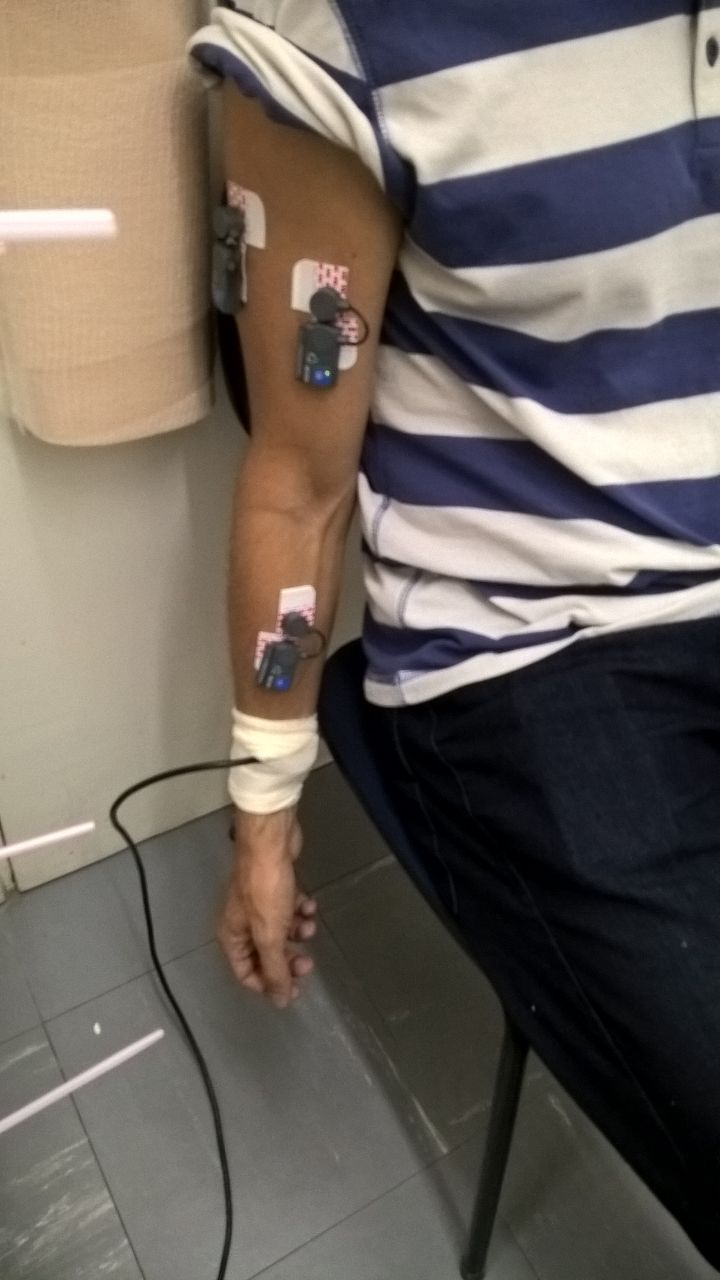
\includegraphics[scale=0.32]{Images/Experiment_Image.jpg}
%       \caption{Experimental setup on a test subject}
%       \label{Experimental Setup}
%    \end{figure}

The subject sat on a chair, with the knees flexed at \(90^{\circ}\), the back perpendicular to the ground with the scapulae pressed against the wall. The posterior part of the upper arm was leaning against a rubber support attached to the wall. This setup guaranteed that the subject was comfortable enough to perform repeated elbow flexions and extensions while maintaining the upper arm steady. 

The experimental protocol had three parts: The first one consisted of an isometric force test to obtain the Maximum Voluntary Contraction (MVC). The elbow of the subject was kept in a fixed position at \(90^{\circ}\) and he/she was asked to apply the maximum possible flexion force. Afterwards, the participant was allowed to rest for a three-minute interval before the next set.

In the second part, the subject was asked to perform five consecutive elbow flexion and extension movements from  \(50^{\circ}\) to \(140^{\circ}\) with a frequency of 0.5Hz. To help the subject reach the correct target angles a template was attached to the wall parallel to the subject, to provide visual guidance. To achieve the desired movement speed a metronome was set at the speed of 60 bpm so that the subject could synchronize the movements with the sound of the metronome. A minute of rest was given to the subject before the next part.

In the third part the subject was asked to make an elbow flexion for 1 second, hold his forearm at \(140^{\circ}\) for 1 s, then a 1 s extension movement and then hold the forearm at \(50^{\circ}\) for another 1 s. This cycle should be repeated five times. Another one minute resting time was given to the subject.
Both of the continuous and interval tests were repeated with 1.5kg and 3kg extra weight placed at the subject's hand.

The test was repeated in a different day, on all test subjects, to further analyze the repeatability of the model proposed in this work. All the data from the tests were transferred to Matlab\textsuperscript{\textregistered} for further analysis and processing.

\subsection{Experimental Data Processing}

The EMG data were pre-processed following procedures described in the literature \cite{Rose20161112,Hayashibe20091621}:
\begin{enumerate}
\item High-pass filtering of the EMG data, using a 2nd order Butterworth filter, with a cutoff frequency of 30 Hz, thus removing noise and artifacts.
\item Full-wave rectification
\item Second Order Butterworth Filter, with 1 Hz cutoff frequency.
\item Normalization with the MVC peak.
\end{enumerate}

This way, the EMG is smoothed and presented as a percentage of the subject MVC instead of Volts.

A low-pass, 20 Hz cutoff frequency, second-order Butterworth filter is applied to the angular data to remove errors and other undesired signals.

Since the position tracking data was sampled at 100 Hz while the EMG data was sampled at 1 KHz, all the position tracking data was resampled to 1000 Hz.
%, an antialiasing finite impulse response (FIR) lowpass filter was applied and the delay introduced by the filter was compensated.

% Figure \ref{Angle and EMG} shows an example of the recorded elbow angle and processed sEMG for the continuous movement with no extra weight.

% \begin{figure}[thpb]
%       \centering
%       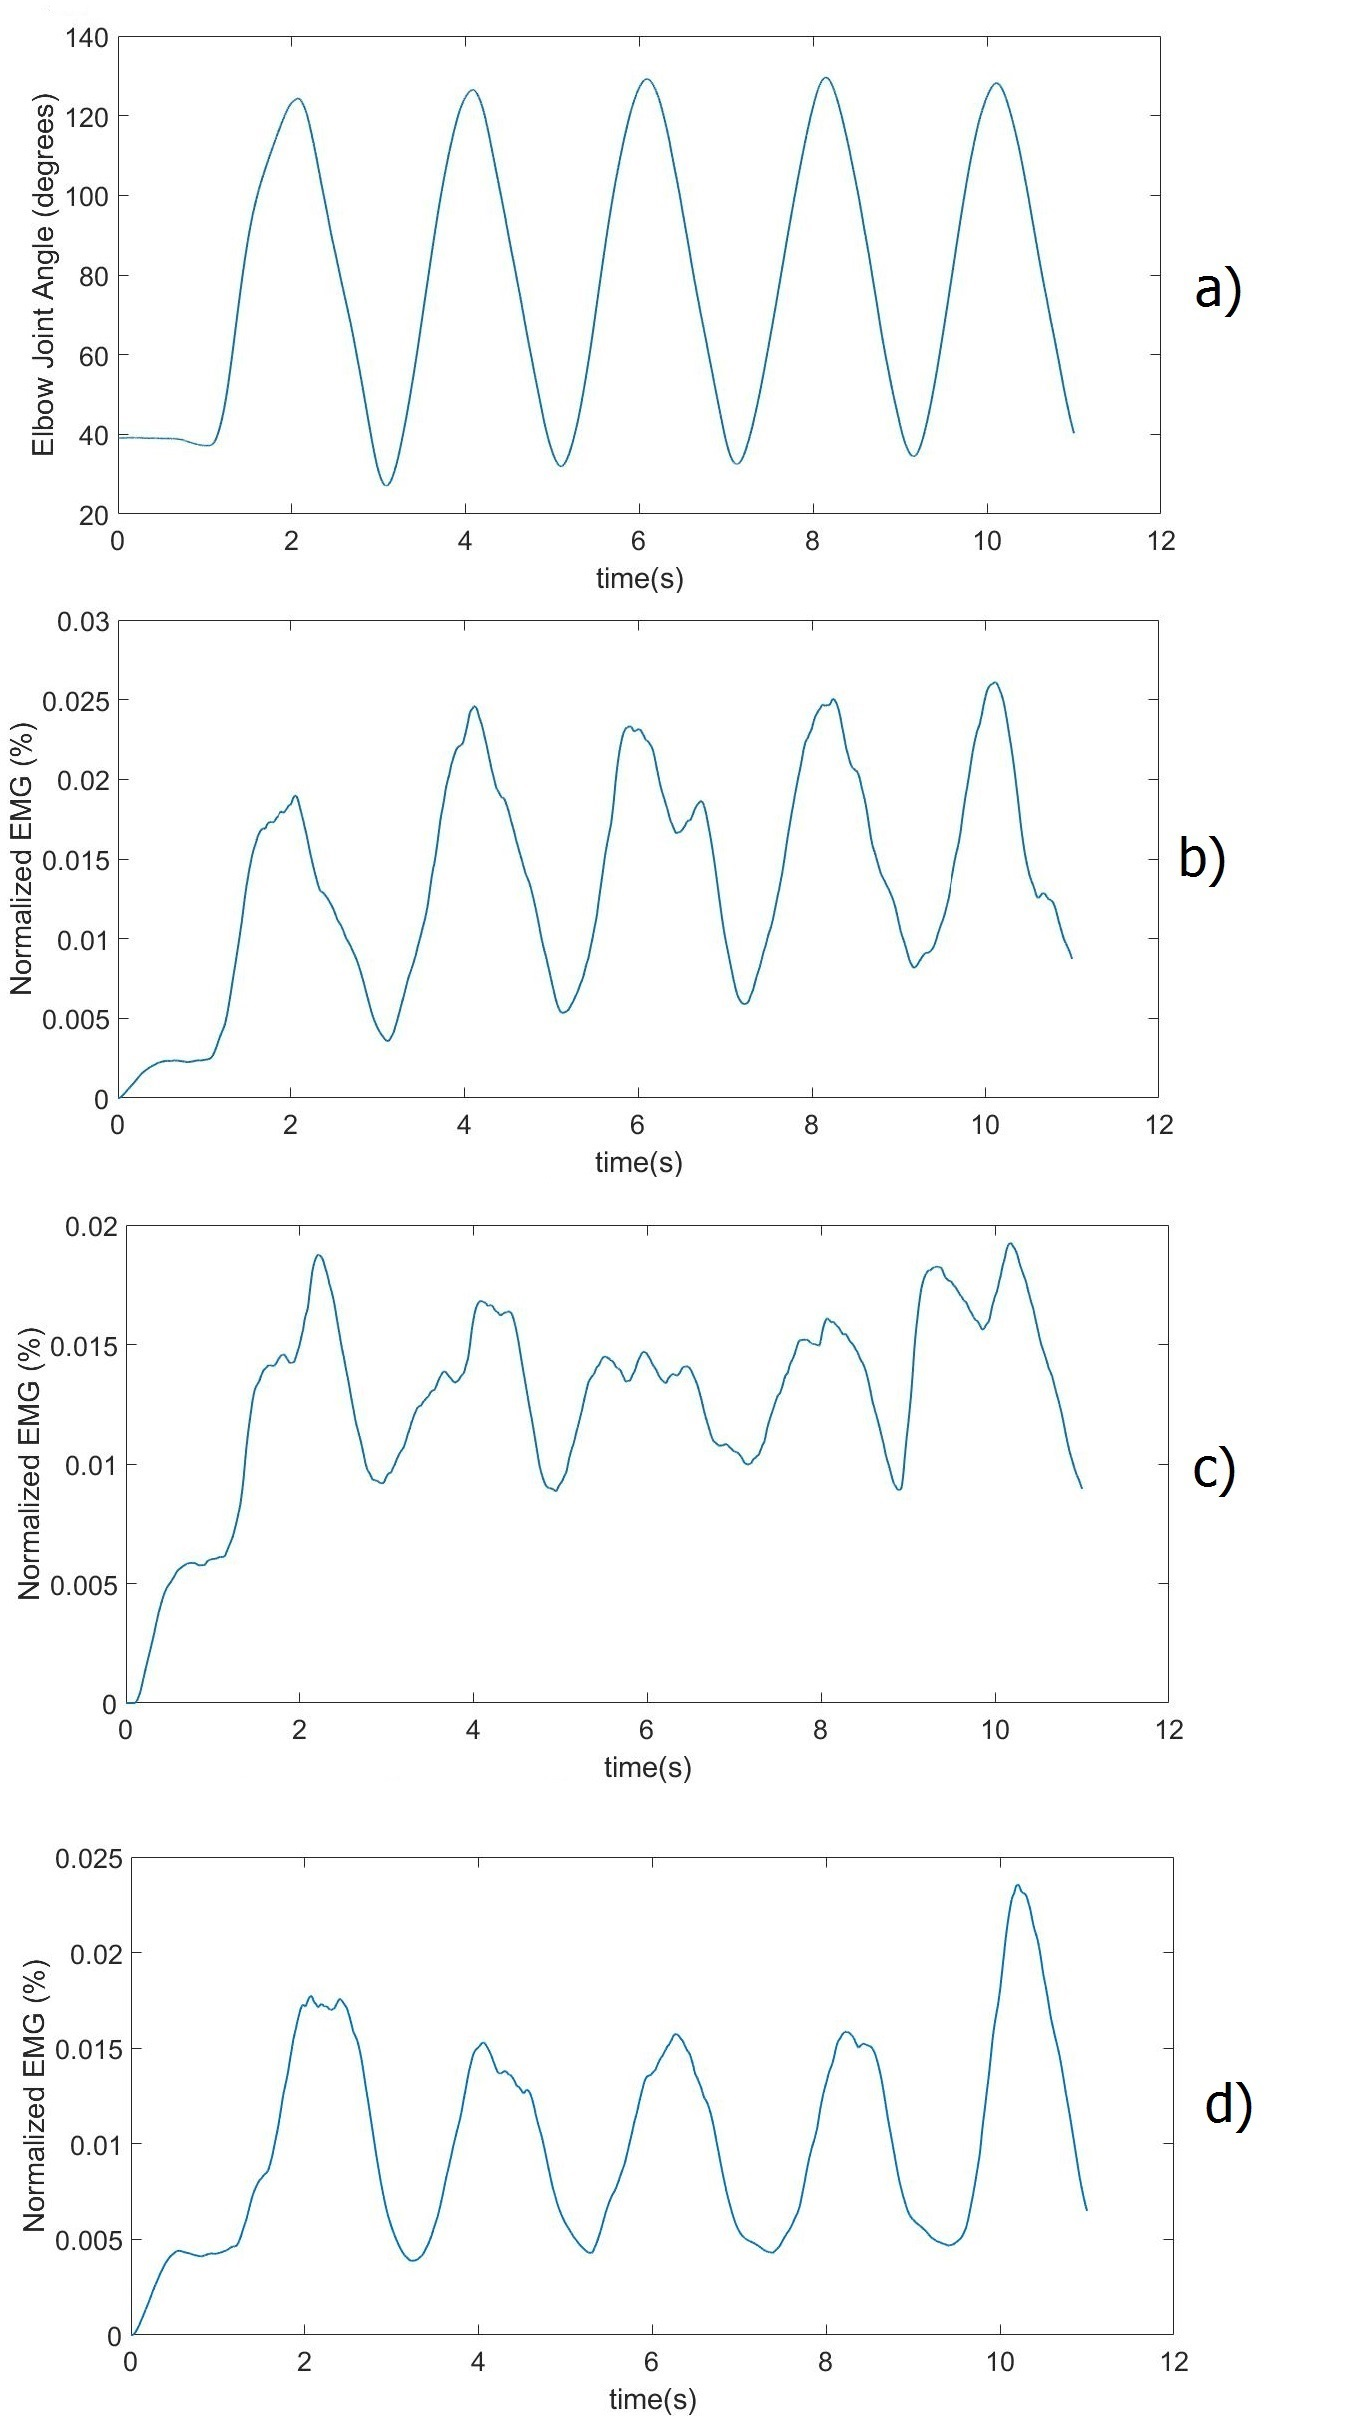
\includegraphics[scale=0.25]{Images/Angle_and_EMGs.jpg}
%       \caption{a) Joint angle for the continuous movement with no extra weight, recorded with the IMU; sEMG values for the b) biceps brachii, c) triceps brachii and d) brachioradialis for the continuous movement with no extra weight. }
%       \label{Angle and EMG}
%    \end{figure}


\section{System Modeling}

\begin{figure}[thpb]
      \centering
      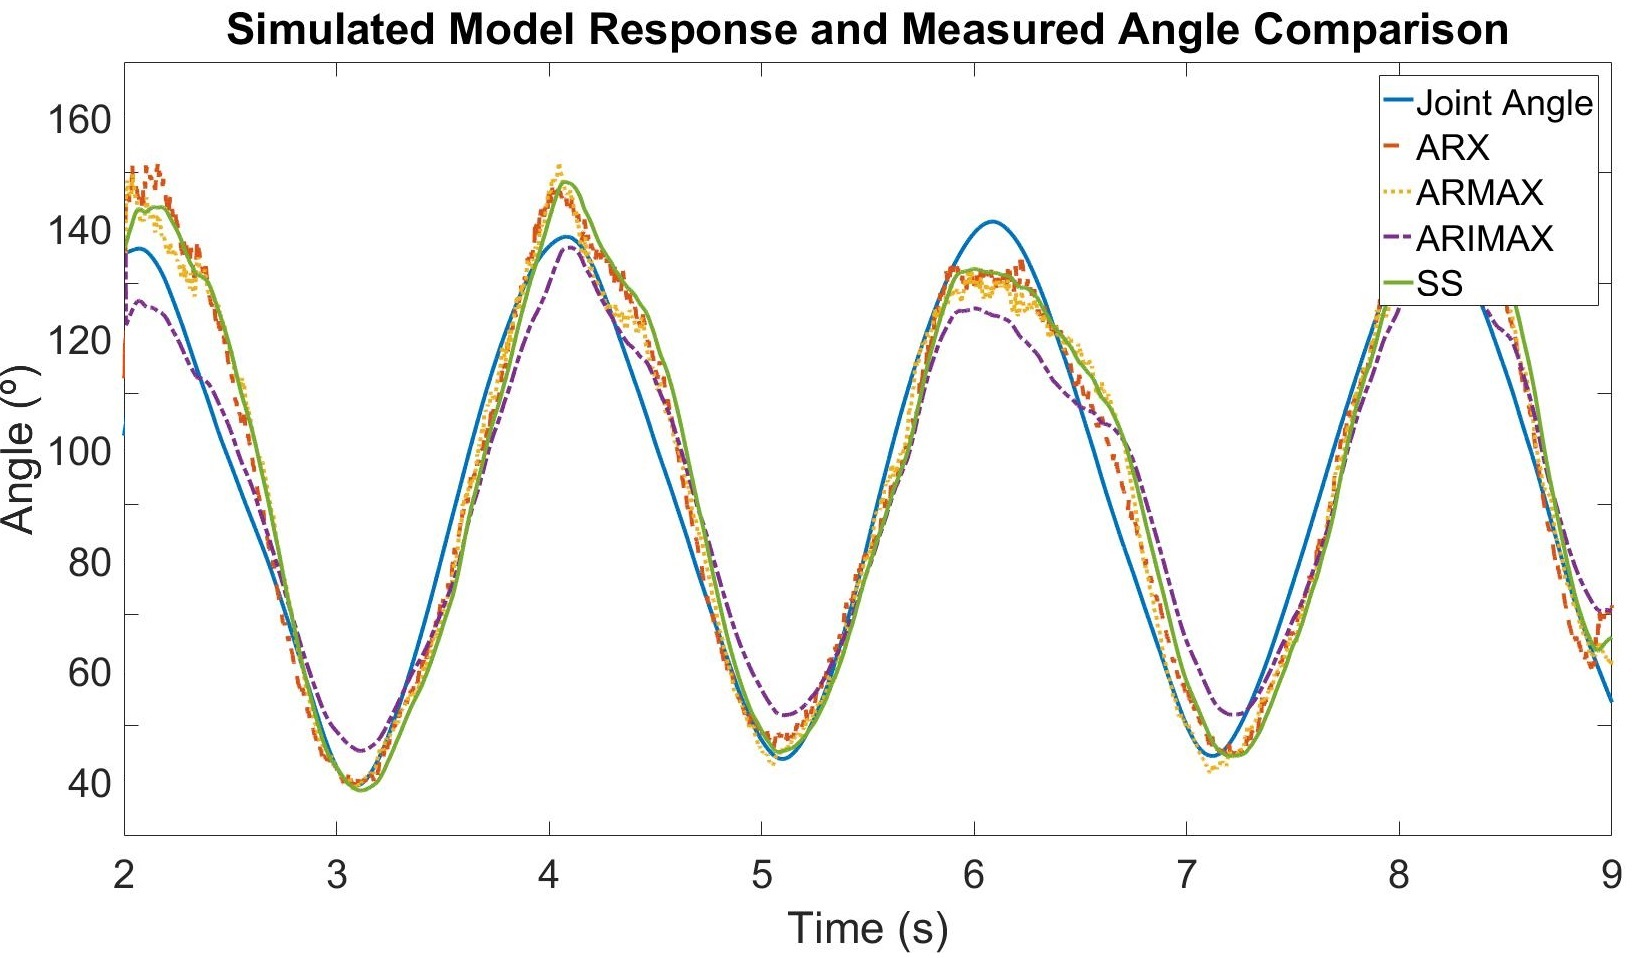
\includegraphics[width=0.95\columnwidth]{Images/simulated_response.jpg}
      \caption{Calculated elbow angle using the models responses compared to the elbow angle measured with the IMU}
      \label{Models Comparison}
   \end{figure}

%It was assumed that the arm model was the same in all the conditions with different inertia values for the different weights attached to the arm of the subject arm. Considering a simple cinematic model of the elbow joint, with one degree of freedom considering the flexion-extension movement in the sagittal plane: 

% * <aforner@usp.br> 2018-01-28T12:41:31.518Z:
% 
% Equation 1: Reviewer said: Joint stiffness is missing.
% 
% 
% ^.

% \begin{equation}
% \label{eq:arm model}
% T = (J + M\cdot L^2)\cdot \ddot{\theta}  + B \cdot \dot{\theta}  + (m\cdot l + M \cdot L) \cdot g \cdot cos(\theta)
% \end{equation}

% Where T is the elbow joint torque, J is the forearm inertia, B is the damping factor of the joint, m is the forearm mass, M is the mass of the dumbbell, g is the gravity force and \(\theta\) is the joint angle. From this simple model it is easy to infer that, by changing the mass of the dumbbell, the arm model parameters also change.



Four different modeling techniques were tested to determine which of them gave the best estimation for elbow angle: Autoregressive with Exogenous Input (ARX), Autoregressive Moving-Average with Exogenous Input (ARMAX), Autoregressive Integrated Moving-Average with Exogenous Input (ARIMAX) and State Space (SS).

In order to find a solution a search was done using 1000 models of each type with random model orders ranging from 1 to 10. A data window of 6s was used to calibrate the model, while the entire data vector was used to validate the model.

Each model was compared to the reference angle using equation \ref{eq:fitness}. The orders of the model that achieved the highest fitness value were chosen and are presented at table \ref{ta:order}. The parameters of the models were estimated using time-domain data in Matlab\textsuperscript{\textregistered}.

% With the model estimation technique chosen, it is necessary to determine the order of its parameters. To determine the chosen model order, 400 random combinations were tested for each data set with order values going from 0 to 10. The order chosen was the one that gave the best fit (see eq. \ref{eq:NRMSE}) between the calculated value and the one measured by the experiment. The coefficients of the models were estimated using time-domain data in Matlab\textsuperscript{\textregistered} (The Mathworks Inc, USA), minimizing a quadratic prediction error criterion.

\begin{equation}
\label{eq:fitness}
Fit = \sqrt[]{\frac{\prod_{i=1}^{3}\prod_{j=1}^{2} Corr_{ij}}{\prod_{i=1}^{3}\prod_{j=1}^{2} RMSE_{ij}}}
\end{equation}

% * <aforner@usp.br> 2018-01-28T12:50:28.105Z:
% 
% Formula might not be consistent with the definition of the normalized root-mean-square error (NRMSE) 
% 
% ^.

% * <leofischi@uol.com.br> 2018-01-29T14:54:45.473Z:
% 
% I am not using NRMSE anymore, only RMSE, described below (eq. (3))
% 
% ^.


Where $Corr_{ij}$ is the correlation between the measured angle and estimated angle for each test; $RMSE_{ij}$ is the Root Mean Square Error between the measured angle and estimated angle (see eq. \ref{eq:RMSE}); $i$ equals 1 for the 0kg test, 2 for the 1.5kg test and 3 for the 3kg test; j equals 1 for the continuous test and 2 for the intermittent test.

\begin{equation}
\label{eq:RMSE}
RMSE = \sqrt[]{mean((y-\hat{y})^2)}
\end{equation}

%\begin{equation}
%\label{eq:RMSE}
%NRMSE = 100*\left(1- \frac{||y-\hat{y}||}{||y-mean(y)||}\right)
%\end{equation}

% * <aforner@usp.br> 2018-01-28T12:52:23.882Z:
% 
% In the formula (3), the definition of q is missing and the dimension of u(t) needs to be clarified, was it a 3-dimensional vector or the formula was actually supposed to be written as B(q)( u_1(t-n_k) + u_2(t-n_k) + u_3(t-n_k))?
% 
% ^.

% * <leofischi@uol.com.br> 2018-01-29T14:58:01.356Z:
% 
% Resolvido
% 
% ^.

Where $y$ is the measured angle and $\hat{y}$ is the estimated angle.
% The chosen method for the modeling of the relationship between elbow joint angle and sEMG was a system identification method called Auto Regressive Moving Average with Exogenous Input (ARMAX). The ARMAX model has the following form:

% For each model, the data acquired from each test subject was separated by weight lifted and the data from the continuous movement and the intermittent movement were merged. This way, it was possible to calculate a single model for the arm movement using the system identification tool in Matlab\textsuperscript{\textregistered}.


\section{Results}

Figure \ref{Models Comparison} shows the comparison between the best models of each type with measured elbow angle for subject 3.

The ARX model outperforms the other models for every subject and every test set. For this reason it was the chosen model for the subsequent estimation procedures.

The ARX model has the following form:

\begin{equation}
\label{eq:ARX}
A(q)\hat{y}(t) = \sum_{m=1}^{3}B_m(q)u_m(t-n_{k_m})+e(t)
\end{equation}

Where \(\hat{y}(t)\) is the output at time t, angle of the elbow joint, in this case; u(t) are the inputs, being the processed sEMG values from biceps brachii, brachioradialis and triceps brachii; e(t) is the white-noise disturbance; \(n_k\)  is the delay for each input; \(q\) is the delay operator; \(m\) equals 1 for the biceps EMG signal, 2 for the triceps EMG signal and 3 for the brachioradialis EMG signal; A and B are the model parameters, defined by:

\begin{equation}
\label{eq:A}
A(q) = 1 + a_1q^{-1}+\dots+a_{n_a}q^{-n_a}
\end{equation}

\begin{equation}
\label{eq:B}
B(q) = 1 + b_1q^{-1}+\dots+b_{n_b}q^{-n_b+1}
\end{equation}


Where \(n_a\) is the number of poles of the system; \(n_b\) is the number of zeros plus one.

The model orders calculated are presented in table \ref{ta:order}.

\begin{table}[h]
\caption{Model orders for each subject}
\label{ta:order}
\centering
\begin{tabular}{|c|c|c|c|}
\hline
 & \(n_a\) & \(n_b\) & \(n_k\)\\
\hline \hline
Subject 1 & 0 & 8, 2, 2 & 1, 2, 2\\
\hline
Subject 2 & 0 & 9, 5, 10 & 1, 3, 0\\
\hline
Subject 3 & 0 & 1, 4, 8 & 5, 0, 1\\
\hline
Subject 4 & 0 & 8, 8, 1 & 0, 0, 8\\
\hline
Subject 5 & 0 & 5, 1, 9 & 2, 8, 0\\
\hline
Subject 6 & 0 & 4, 3, 10 & 3, 0, 0\\
\hline
\end{tabular}
\end{table}

\begin{figure}[thpb]
\vspace{2mm}
      \centering
      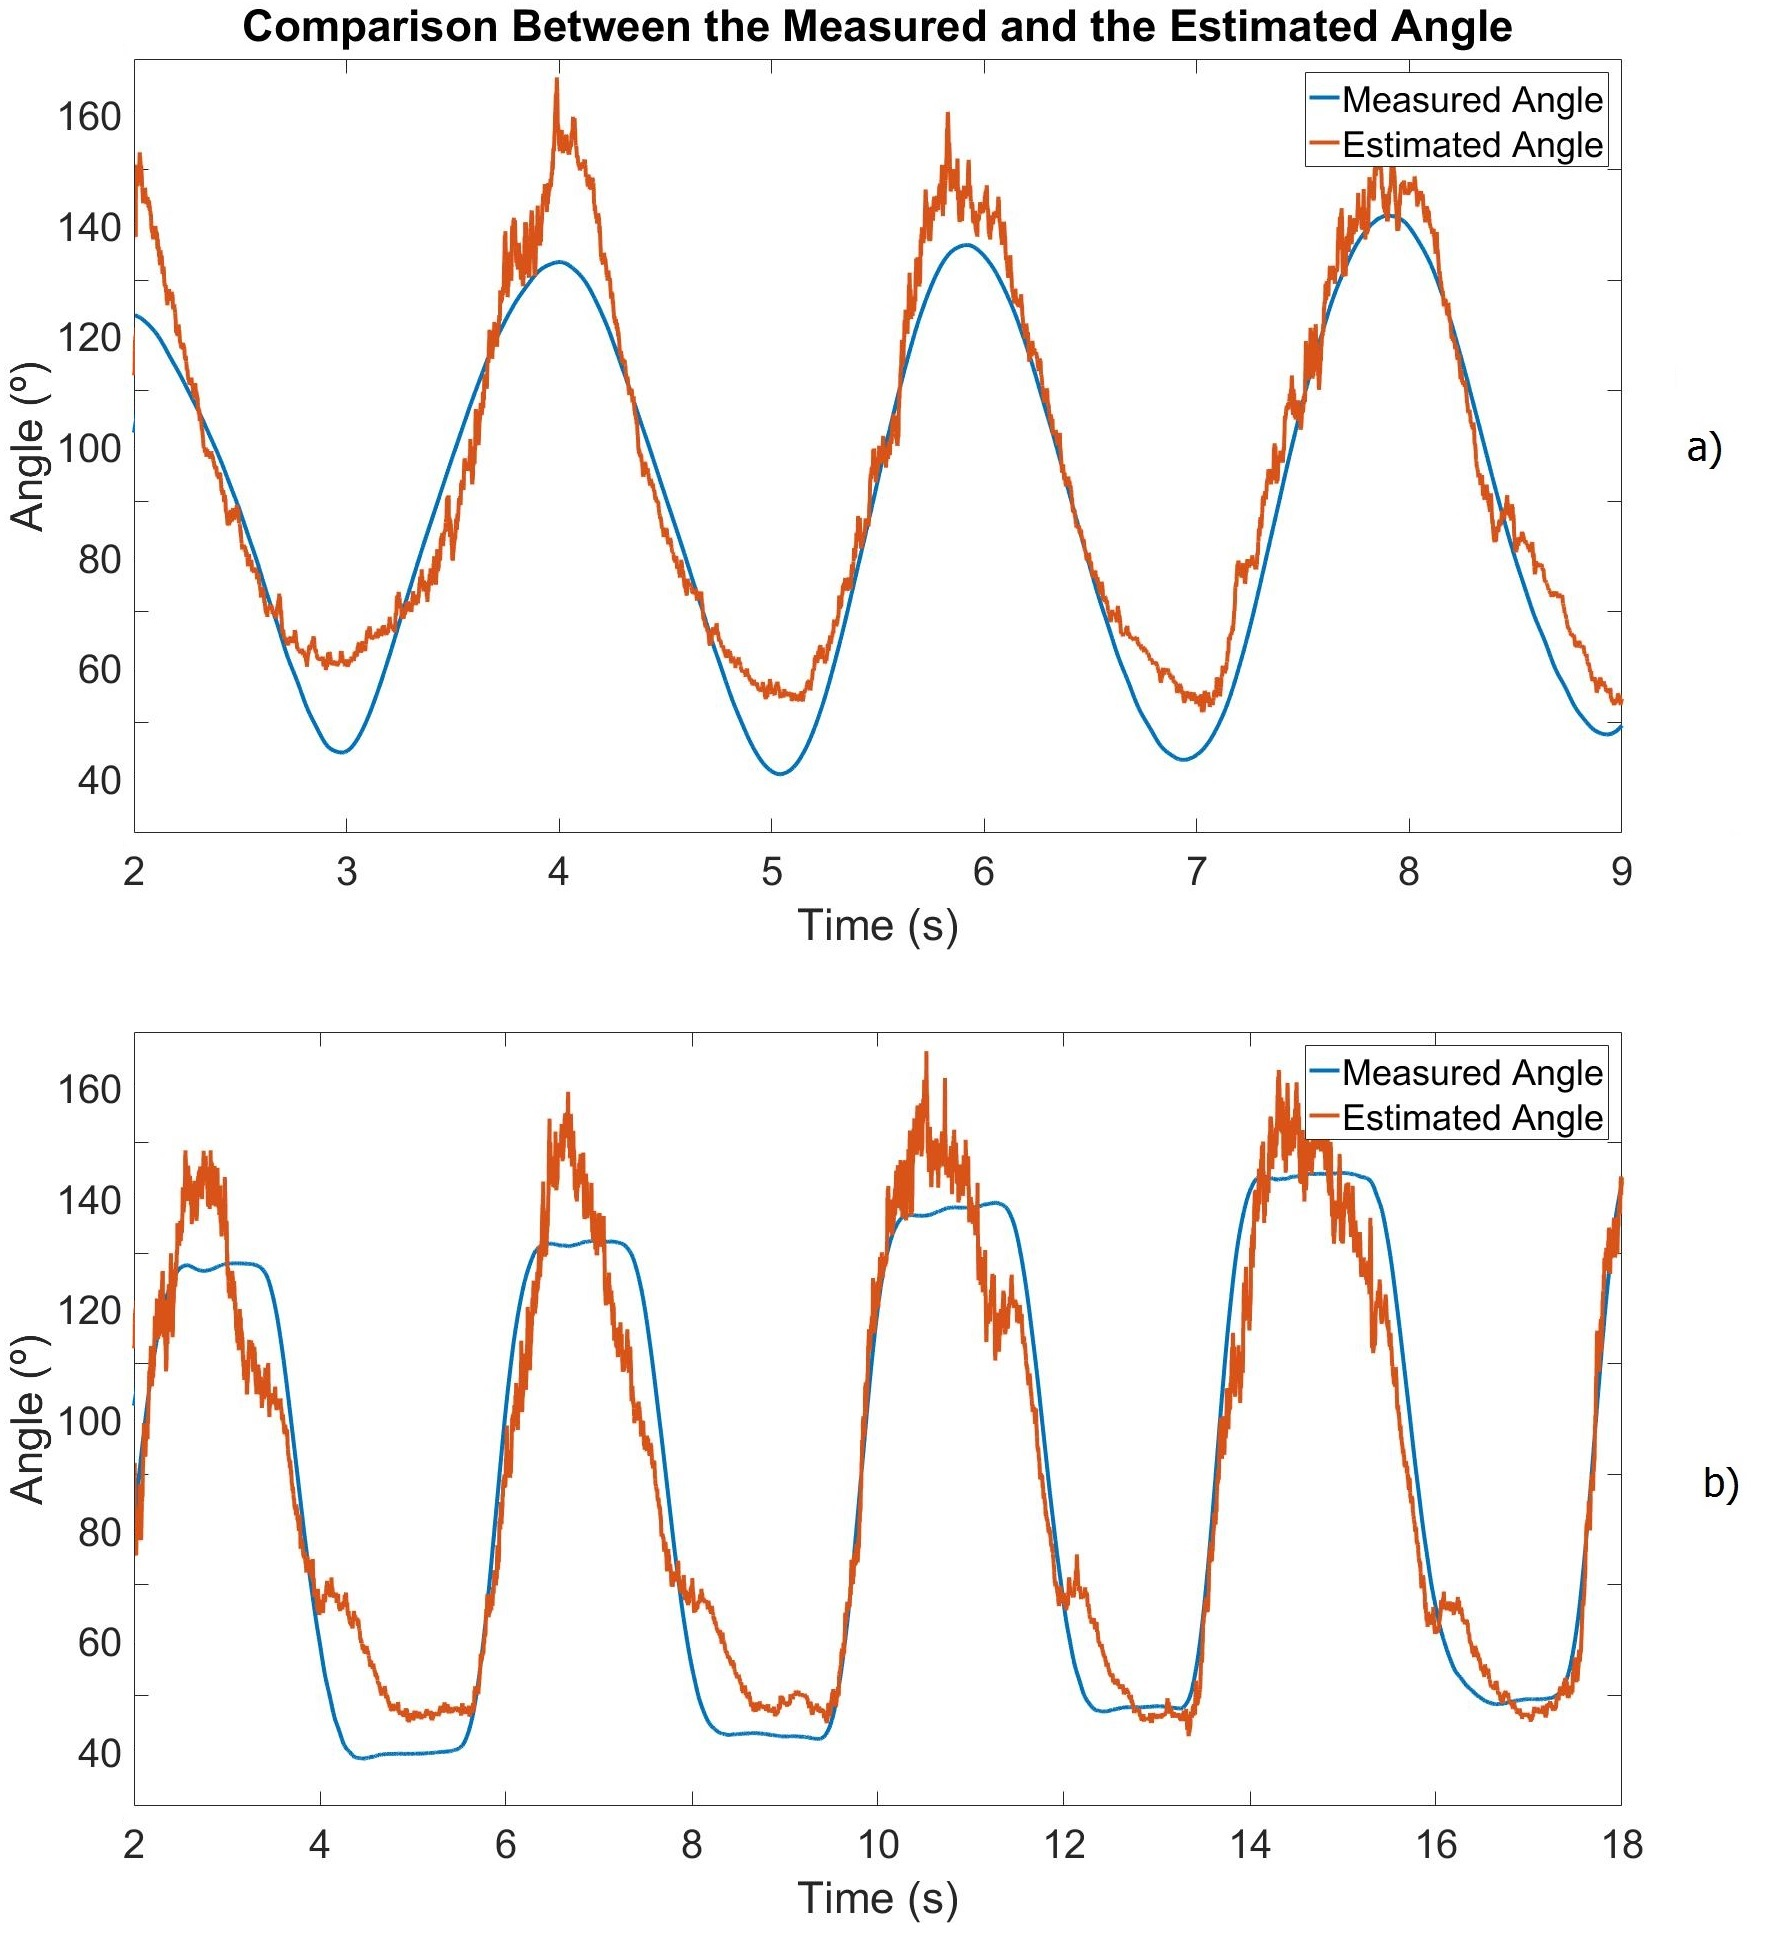
\includegraphics[width=0.98\columnwidth]{Images/comparison.jpg}
      \caption{Comparison between the measured angle of the elbow joint and the angle calculated through the use of the estimated model, for subject 2, with a 1.5kg dumbbell. a) shows the comparison for the continuous movement and b) the comparison for the discrete movement}
      \label{Angle Comparison}
   \end{figure}
   

Using the values from table \ref{ta:order} as the ARX model orders, it was possible to calculate the model for elbow joint angle using the three sEMG measurements as input and compare it to the experimentally measured values. As an example, figure \ref{Angle Comparison} shows a comparison between the calculated and estimated angle, for continuous and intermittent movement.

Using the same model parameters previously calculated, we estimated the response of the system using a second batch of data, recorded in a different day. %An example of the result of this process can be seen in figure \ref{Validation Procedure}, where the model calculated for the subject number 3 was used to estimate the elbow joint angle using the input data acquired from the second day of testing.
The data acquired from the second experimental set were also used to calculate a new model, using the same model orders determined in the first experimental set. This way, it is possible to evaluate if the model orders calculated in one test set can be used to calculate a new model from a different data set.

   
   \begin{table*}[t]
   \vspace{2mm}
\caption{Correlation factor and Root-mean-square error for the calculated and measured angle values}
\label{ta:correlation}
\centering
\resizebox{0.99\textwidth}{!}{%
\begin{tabular}{|c c|c c|c c|c c|c c|c c|c c|}
\hline
\multicolumn{2}{|c|}{} & \multicolumn{4}{c|}{Model Estimation, first test set} & \multicolumn{4}{c|}{Same model, second test set} & \multicolumn{4}{c|}{New model, same orders, second test set} \\
\hline
\multicolumn{2}{|c|}{} & \multicolumn{2}{c|}{Continuous} & \multicolumn{2}{c|}{Intermittent} & \multicolumn{2}{c|}{Continuous} & \multicolumn{2}{c|}{Intermittent} & \multicolumn{2}{c|}{Continuous} & \multicolumn{2}{c|}{Intermittent} \\
\hline
\multicolumn{2}{|c|}{} & Correlation & RMSE (degrees) & Correlation & RMSE (degrees) & Correlation & RMSE (degrees) & Correlation & RMSE (degrees) & Correlation & RMSE (degrees) & Correlation & RMSE (degrees)\\
\hline \hline

& 0 kg &0.9477 &13.73 &0.9404 &17.36 & 0.0224 & 65.02 & 0.1546 & 60.29 &0.9500 &10.84 & 0.8195 &20.76\\
Subject 1 & 1.5 kg &0.9615 &13.21 &0.8042 & 24.30 &0.8067 &17.06 & 0.7250 & 18.50 &0.9458 &7.959 &0.7118 &18.79 \\
& 3 kg &0.9764 &12.30 &0.8994 &18.10 & 0.9322 & 17.23 & 0.8624 & 16.80 &0.9381 &12.64 &0.8454 &14.47\\
\hline

& 0 kg &0.9163 &14.32 &0.9070 &17.27 & 0.8113 & 32.33 & 0.9089 & 21.53 &0.9543 &11.59 &0.9251 &13.64\\
Subject 2 & 1.5 kg &0.9707 &9.715 &0.9585 & 11.50 & 0.7685 & 23.11 & 0.8647 & 18.06 &0.9544 &12.20 &0.9062 &14.65\\
& 3 kg &0.9329 &18.56 &0.9494 &12.83& 0.8715 & 21.50 & 0.9419 & 16.88 &0.9294 &12.15 &0.9481 &11.60\\
\hline

& 0 kg &0.9766 &9.464 &0.9349 &16.67 & 0.9667 & 19.69 & 0.9078 & 15.78 &0.9810 &20.01 &0.9218 &14.62\\
Subject 3 & 1.5 kg &0.9634 &13.77 & 0.9316& 13.06 & 0.9417 & 12.66 & 0.9126 & 16.01 &0.9622 &11.28 &0.9078 &16.50\\
& 3 kg &0.9345 &16.67 &0.9382 &13.78& 0.9470 & 13.05 & 0.9363 & 14.43 &0.9672 &13.27 &0.9355 &14.51\\
\hline

& 0 kg &0.8847 &18.46 &0.8891 &19.72 & 0.1142 & 78.67 & 0.1388 & 56.36 &0.9254 &15.57 &0.9213 &18.62\\
Subject 4 & 1.5 kg &0.9463 &17.95 &0.9147 &18.23 & 0.7432 & 36.97 & 0.7774 & 38.19 &0.8878 &18.77 &0.8045 &23.43\\
& 3 kg &0.9329 &21.59 &0.8744 &18.40 & 0.8785 & 79.74 & 0.8508 & 29.37 &0.9106 &17.12 &0.9074 &20.04\\
\hline

& 0 kg &0.9030 &17.28 &0.8381 &25.19 & 0.9489 & 26.50 & 0.8732 & 17.82 &0.9616 &11.41 &0.9031 &19.40 \\
Subject 5 & 1.5 kg &0.8336 &18.24 &0.7901 &21.25 & -0.6302 & 58.17 & -0.6882 & 70.69 &0.9246 &15.89 &0.9028 &13.29\\
& 3 kg & 0.8989 &20.56 &0.8347 &24.23& 0.9499 & 97.20 & 0.9264 & 104.2 &0.9772 &15.77 &0.9295 &11.11\\
\hline

& 0 kg &0.9408 &15.91 &0.9089 &19.34 & 0.9504 & 41.71 & 0.9066 & 46.66 &0.9528 &15.21 &0.9180 &17.30\\
Subject 6 & 1.5 kg &0.9406 &22.16 &0.9468 &15.91 & 0.8456 & 75.72 & 0.8487 & 87.73 &0.8572 &17.29 &0.8812 &18.10 \\
& 3 kg & 0.8798 & 19.65 &0.8863 &18.88 & 0.8272 & 58.04 & 0.8220 & 54.78 &0.8740 &17.39 &0.8725 &17.10\\
\hline


\end{tabular}%
}
\label{ta:corr}
\end{table*}

To better determine the accuracy of the model, two performance parameters were used: correlation coefficient and the root-mean-square error (RMSE) between the estimated and the measured elbow joint angles. Table \ref{ta:corr} shows the accuracy performance parameters for each participant and every test set. The different results for each method described above are presented in columns. The first data set was used to obtain a model that was used to estimate the joint angles that were compared to the measured angle values. Afterwards, the model obtained from the first experimental set was used with the sEMG inputs from the second experimental set to estimate the corresponding joint angles. Finally, using the same model orders chosen from the first data set, a new set of model parameters was obtained from the second data set, and the output was compared to the measured angle data.


\section{Discussion}

This paper proposed a method to estimate the elbow joint angle based on the measurement of the sEMG of biceps brachii, triceps brachii and brachioradialis. The sEMG-to-Angle model was estimated using the data collected from experiments and a system identification method, more specifically, ARX. With the acquired sEMG data as input to the estimated model, it was possible to estimate the elbow angle. Using the data from the IMU it was possible to validate the estimation based on sEMG acquired from six participants during two experimental sessions in different days.

% \begin{figure}[bthp]
%       \centering
%       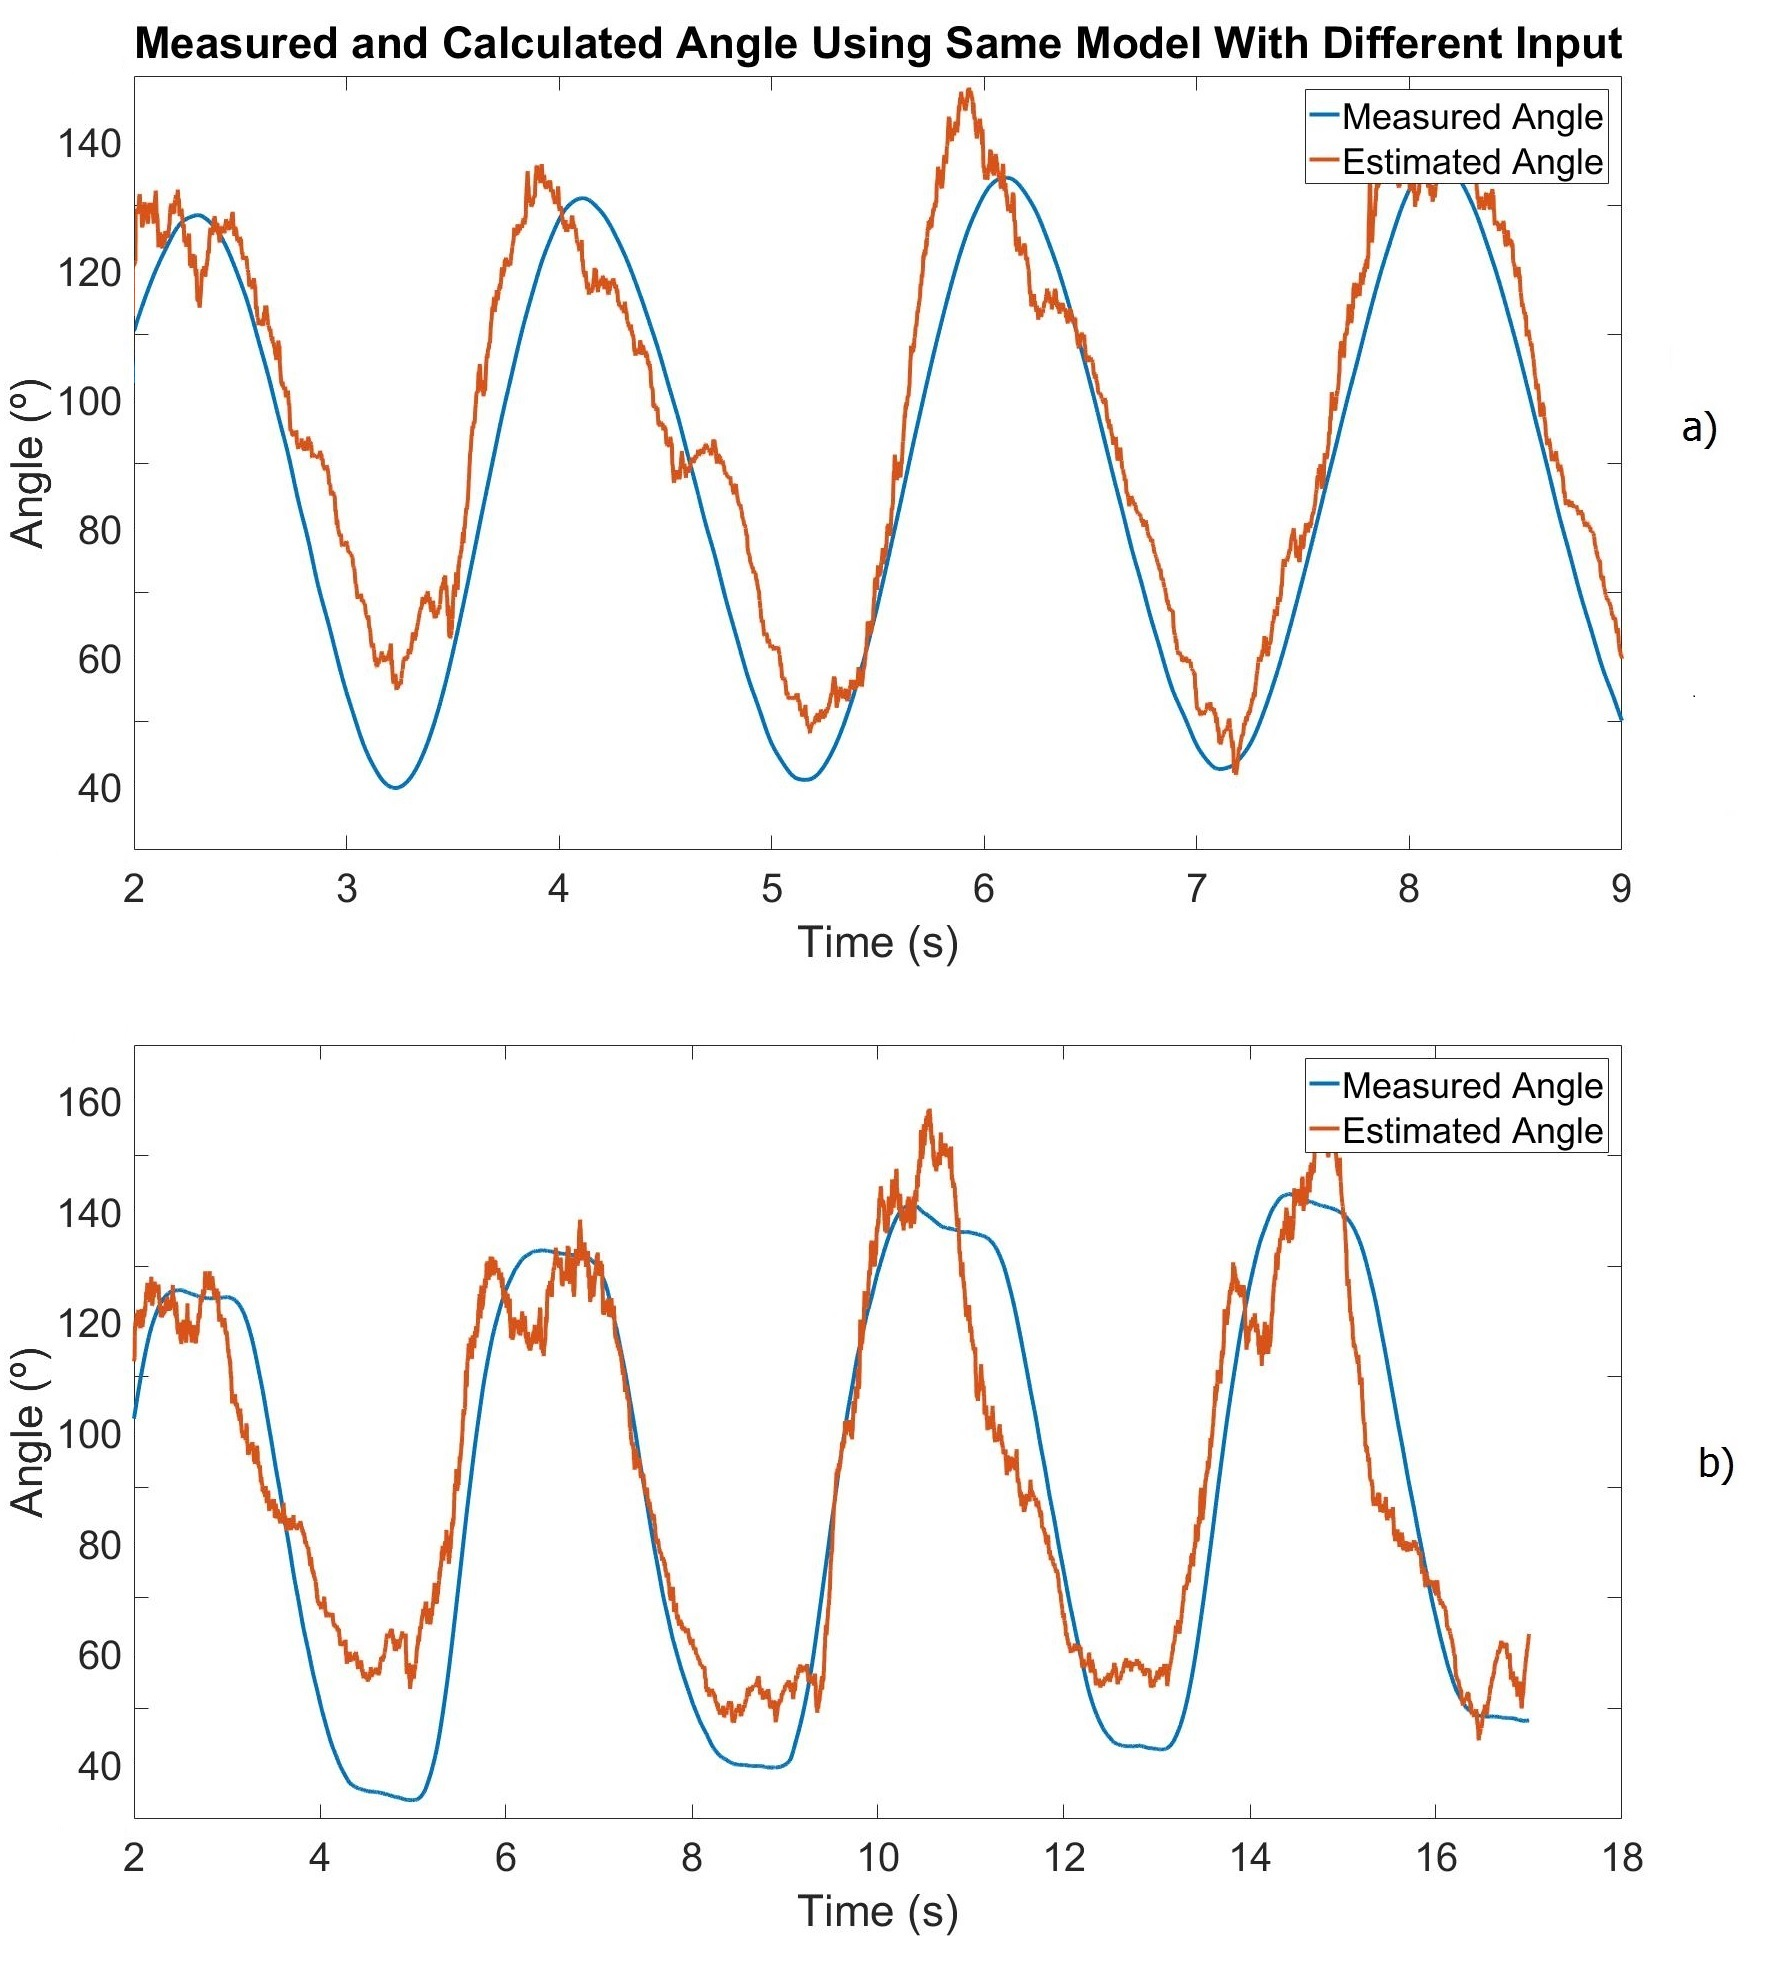
\includegraphics[width=0.95\columnwidth]{Images/Different_Input.jpg}
%       \caption{Using the same model calculated with the first data set, but using the EMG data from the second test set as input. a) shows the comparison for the continuous movement and b) the comparison for the discrete movement}
%       \label{Validation Procedure}
%    \end{figure}

The experimental data showed that it is possible to use the EMG data to estimate joint angles from sEMG values for the experimental conditions presented here. %Even though estimating one model for continuous movement and another one for discrete movement gives higher precision, it is possible to calculate a single model for both movements.
The results achieved in this paper show similar precision values to those achieved by other authors  \cite{Pang2015165,Liu1999391,Rahmatian2016158,Mamikoglu2016785}. For most of the simulations, the model achieved correlations above $90\%$ and RMSE under $20^\circ$. Considering the worse results, the correlation was above $70\%$ and the RMSE lower than $25^\circ$.

%As stated before, by lifting different weights the model parameters are altered. For the same test subject the A(q) and C(q) parameters (see eq. 3) maintained values with less than 1\% difference from one another, while the B(q) values assumed a greater range of values.

%Even for different subjects, the estimated A(q) and C(q) parameters also had a difference of less than 1\% from one another.

%From the seven subjects, six of them could be estimated by an ARMAX model with the same parameters order. The test subject with different order parameters was the one that presented the worst readings of the brachioradialis muscle EMG. Because of that, a lot of noise is introduced, requiring a higher order system to overcome the modeling errors. The brachioradialis is the most difficult muscle to read the sEMG signals compared to the biceps brachii and the triceps brachii. This difficulty is due to the muscle short length causing the electrodes to stay close to the tendon, which induces  reading errors. Not coincidentally, this test subject was the one with smaller stature.

%The repeatability of the model was successful for the cases studied in this work, even though it is possible to note that the model is not as precise as it was for the calibration procedure.

For the majority of the test subjects, it was not possible to use the same model to estimate the angle of the elbow joint for tests conducted in different days. One way to address this problem would be to rescale the output signal to the angle range, minimizing the RMSE of the output signal. Since the EMG signals may change for one time to another, due to several reasons as slight change in electrode position, tissue properties or temperature \cite{soderberg1975}, it may not be possible to determine a model that estimates the joint angle for data acquired on different days or test setups, using the methods described in this work. With this in mind, a solution would be to recalibrate the model at each session.

\addtolength{\textheight}{-4.5cm} % This command serves to balance the column lengths
                                  % on the last page of the document manually. It shortens
                                  % the textheight of the last page by a suitable amount.
                                  % This command does not take effect until the next page
                                  % so it should come on the page before the last. Make
                                  % sure that you do not shorten the textheight too much.

For subjects 2 and 3, repeating the model achieved correlation above $75\%$ and RMSE below $32^\circ$. For subject 3, specifically, using the same model achieved values of correlation above $90\%$ and RMSE below $20^\circ$. Even though it is possible to note that the estimation is not as precise as it was when using the first data set as input, these results can be regarded as very good compared to other similar works. More investigation is required to determine if those models are capable of estimating the joint angle for any test conducted with these test subjects.
% * <aforner@usp.br> 2018-01-28T12:57:50.848Z:
% 
% > good
% Whats is good? Give a value.
% Suggestion: "...correlation above XXX and RMSE below YYY that can be regarded as very good compared to other works... REF."
% 
% ^.

% * <leofischi@uol.com.br> 2018-01-29T17:47:47.336Z:
% 
% Resolvido
% 
% ^.

The same model order calculated in the first test can be used for the subsequent test sessions, without a reduction in the accuracy of the predicted angle. This shows that, even considering that environmental noise affects the EMG signal, it does not change the system order. With the model orders already calculated, a recalibration procedure can be quickly applied, minimizing the problem of model non-repeatability.

In future work we will analyze if it is possible to estimate one model for each subject that does not depend on the weight. Moreover, it would be very interesting to obtain a subject-independent model that can estimate joint angles for a large group of subjects. These models will be used for the control of an EMG-driven upper limb exoskeleton.


%%%%%%%%%%%%%%%%%%%%%%%%%%%%%%%%%%%%%%%%%%%%%%%%%%%%%%%%%%%%%%%%%%%%%%%%%%%%%%%%

%%%%%%%%%%%%%%%%%%%%%%%%%%%%%%%%%%%%%%%%%%%%%%%%%%%%%%%%%%%%%%%%%%%%%%%%%%%%%%%%

%%%%%%%%%%%%%%%%%%%%%%%%%%%%%%%%%%%%%%%%%%%%%%%%%%%%%%%%%%%%%%%%%%%%%%%%%%%%%%%%

%%%%%%%%%%%%%%%%%%%%%%%%%%%%%%%%%%%%%%%%%%%%%%%%%%%%%%%%%%%%%%%%%%%%%%%%%%%%%%%%


\bibliography{biblio_EMG_Joint}
\bibliographystyle{unsrt}


\end{document}
